\chapter{Introduction}

    In this first chapter we introduce \emph{developer expertise} in Section~\ref{sec:intro}, then uncover the motivation behind this work in Section~\ref{sec:motivation}. Motivation will be followed up by our \emph{research questions} that we seek to find answers to in Section~\ref{sec:RQs}, then our \emph{contributions} will be following in Section~\ref{sec:contribution}, and lastly a \emph{thesis structure} will conclude this chapter in Section~\ref{sec:thesis_structure}.
    
    \section{Developer Expertise\label{sec:intro}}
    
        In today's world, one can argue that software development is a competitive field. Technology giants such as Google, Facebook, Amazon, Microsoft and Apple have virtually unlimited resources to achieve their goals by releasing newer, faster, and better software than their direct competition. One might ask what is their secret? We subjectively believe that one of their secrets lies in the hard-working, talented people that they hire. Ian Sommerville writes in a book about \emph{Software Engineering} that bad hiring decisions are one of the main risk factors when aiming to build a successful software \cite{sommerville2016software}. Smaller companies and start-ups do not start with equal chances against the technology giants, as they do not possess the same financial and human resources. We argue that in order to maximize the likelihood of building the best possible software, the key is in \emph{hiring the right expert developers} who are a perfect fit for their position. The technology giants have thousands, even millions of applicants each year. For instance, in 2014 it was reported that Google received about three million applicants per year \cite{nisen_2014}, and only the best of the best \emph{the experts} get hired. Becoming an expert developer is probably the goal of every one of those applicants. Finding the right expert for a job opening is certainly the goal of every recruiter and HR manager, but it is difficult to determine the actual expertise of developers just from reviewing their CVs or resumes.
    
    \section{Motivation\label{sec:motivation}}
        A few problems arise when the concept of expertise is put into application: how does one know if they are an expert in something, how can developer expertise be defined, measured, extracted or even learnt? The main motivation of this work is answering some of the above questions that come up as barriers to the implementation of expertise-driven applications. Previous research work had similar motivations, as the problem of finding experts, defining and learning developer expertise from data is a popular problem in software engineering. Mockus and Herbsleb \cite{mockus2002expertise} presented one of the first tools attempting to quantify expertise performance. Baltes and Diehl \cite{baltes2018towards} noted how difficult it is to propose objective quantitative measures of expertise. Teyton et al. \cite{teyton2013find} attempted to detect third party library experts in open source software communities. The authors were motivated by the fact that modern software depends on numerous third-party libraries and developers require substantial expertise to maintain their software systems.
        
        \label{LinkedIn_flaws}One might ask, why research developer expertise when social platforms such as \emph{LinkedIn}\footnote{\url{https://www.linkedin.com}} or job search engines such as \emph{Indeed}\footnote{\url{https://www.indeed.com}} exist. \emph{LinkedIn} recommends job advertisements to users, facilitates faster and more convenient ways to apply for positions, and allows recruiters to post job opportunities and have applicants apply for positions. \emph{LinkedIn} users can enter their previous work experiences, display their top skills, and most importantly the online platform will compute similarity scores between pairs of users and job advertisements, then rank the user compared to other candidates and recommend top candidates for the recruiter to hire. One might say \emph{LinkedIn}'s recommender systems act as an automated expert candidate detector, but that is not the case. One essential factor on \emph{LinkedIn} is that users self-report their education, previous experience, and top skills. This means that users can lie about their education or previous work experiences, exaggerate their skills, neglect some skills, and even add skills that they do not possess. Thus, \emph{LinkedIn}'s recommender systems are as accurate as the information self-reported by users, and it is questionable how much a recruiter should rely on the candidates recommended by \emph{LinkedIn} actually being the top candidates.
        
        \subsection{Developer Expertise in Collaborative Platforms}
            Greene and Fischer \cite{greene2016cvexplorer} have expressed similar concerns about \emph{LinkedIn}, and suggested expanding the candidate search to developer-oriented platforms, such as GitHub\footnote{\url{https://github.com/}} and Stack Overflow\footnote{\url{https://stackoverflow.com/}}, noting that it could become valuable for the recruitment process. Greene and Fischer also mentioned that identifying and hiring candidates with proper skills is necessary for a software project to succeed. Hauff and Gousios \cite{hauff2015matching} had very similar motivations in their work suggesting matching job advertisements to developers, based on developer activity extracted from their GitHub profiles. Tian et al. \cite{tian2019geek} had very similar intentions when they proposed the recommendation of expert developers using user behaviour and contributions on GitHub and Stack Overflow.
            
            One can notice a pattern of leveraging data from collaborative platforms, such as GitHub and Stack Overflow, to learn the expertise of developers based on their software development related activities on the platform. These collaborative platforms are online communities containing question answering, discussion and shared source code related activities \cite{wang2018survey}. These platforms provide a way for developers to communicate and collaborate with their peers while gaining and sharing knowledge. Tian et al. \cite{tian2019geek} state that the success of question answering platforms highly depends on the number of expert users who contribute regularly by answering questions, suggesting more efficient algorithms and pointing out flaws in source code. Greene and Fischer \cite{greene2016cvexplorer} explained that collaborative platforms are an excellent source of data for identifying the right candidate for a job opening, as content on such platforms tend to contain large amounts of technical information, thus developer interest and expertise can be inferred with the help of text mining algorithms and language models. Zhang et al. \cite{zhang2014recommending} confirmed Greene and Fischer's claims, as they stated that user behaviour is a rich source of data about the software development process. Tian et al. \cite{tian2019geek} explored the benefits of cross-platform expert recommendation systems, and they referred to GitHub and Stack Overflow as the primary data source for such a system. They stated that such a cross-platform system could shed a light on what professional activities are conducted by various types of users. 
            
            While there are numerous advantages of being part of communities on collaborative platforms, Wang et al. \cite{wang2018survey} outlined a few challenges that these platforms have: 1) Popular collaborative, question answering platforms get thousands of new questions daily, while there could be millions of already existing questions on the platform. The very large volume of questions makes it difficult for a contributor to decide which questions to answer; 2) Contributors tend to have various interests and expertise in different areas of their field, so the quality of the answers could be inconsistent, and 3) some questions do not receive an answer on the same day, thus some users will have to wait for long periods to get a satisfactory answer. 
            This being said, the main motivations behind learning developer expertise from collaborative platforms are: 1) to find out whether developer expertise could be accurately extracted and learnt from collaborative platforms, 2) to investigate if users maintain similar expertise profiles across multiple collaborative platforms, and 3) to develop one or more novel techniques to extract developer expertise areas from collaborative platforms.
            
             \begin{figure}[!ht]
                  \centering
                  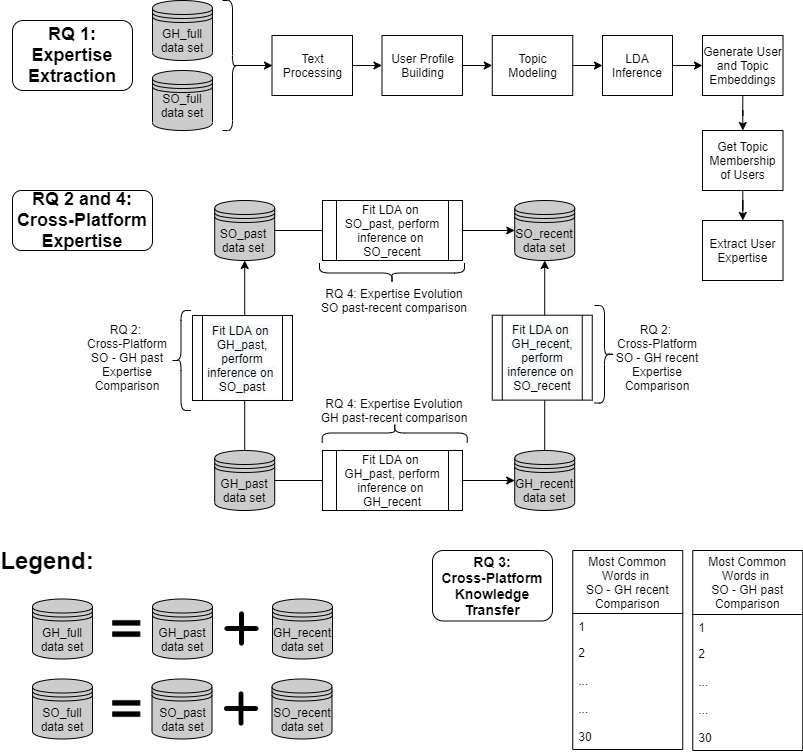
\includegraphics[width=\textwidth]{figures/roadmap.jpg}\\
                  \caption{Our research roadmap.}
                  \label{fig:roadmap.jpg}
            \end{figure}
    
    \section{Research Questions\label{sec:RQs}}

        Figure~\ref{fig:roadmap.jpg} presents the overall research roadmap that connects our research questions with the methodology we followed. We address the following research questions in our work:
       
        \begin{itemize}
            \item \textbf{RQ1: How can we extract the major expertise areas of Stack Overflow and GitHub users? How do expertise trends compare on Stack Overflow and GitHub?}
            
            This research question is addressing the unknown behind quantitative developer expertise: how to define, extract, measure and rank expertise of Stack Overflow and GitHub users. This research question is extremely important, as it drives the search for novel, data-driven techniques that can accurately extract expertise from software artifact related data. Once expertise has been extracted, a follow-up question will focus on comparing the newly discovered trends from Stack Overflow and GitHub.
            
            \item \textbf{RQ2: How similar are developer expertise profiles in two different collaborator platforms, Stack Overflow and GitHub?}
            
            This research question is intended to provide a comparative expertise analysis between the two different collaborative platforms, i.e., Stack Overflow and GitHub, to allow software engineers to understand how similar or different are the expertise profiles on the two platforms. This insight could expend our understanding of cross-platform developer expertise.
            
            \item \textbf{RQ3: What knowledge is transferable from one platform to another?}
            
            This research question builds further analysis on top of RQ2 by analyzing what are the similarities between the two platforms and what kind of knowledge is the most transferable from one platform to another. Getting insight into knowledge transfer would allow software developers to understand what skills could be learned by using both Stack Overflow and GitHub.
            
            \item \textbf{RQ4: How does developer expertise evolve on Stack Overflow and GitHub?}
            
            This research question focuses on the change in expertise over time and it is intended to explore and better understand the expertise evolution on Stack Overflow and GitHub. This final research question is important in order to understand if people are improving their skills, or whether they gain new skills.
        \end{itemize}
        
    \section{Contributions\label{sec:contribution}}
        The contributions made in this line of research are 7-fold:
        \begin{itemize}
            \item Development of three novel techniques to extract developer expertise topics from Stack Overflow and GitHub (\emph{RQ1})
            \item Analysis of developer expertise trends on Stack Overflow and GitHub (\emph{RQ1})
            \item Comparison of developer expertise across two collaborative platforms (\emph{RQ2})
            \item Empirical evidence about knowledge transfer between two collaborative platforms (\emph{RQ3})
            \item Analysis of developer expertise evolution trends from two collaborative platforms (\emph{RQ4})
            \item Collection of developer expertise ground truth data set
            \item Development of four new data sets (\emph{GH-past and recent, SO-past and recent}) by aggregating Stack Overflow and GitHub data.
        \end{itemize}
    
     \section{Thesis Organization\label{sec:thesis_structure}}
        The structure for the rest of this thesis is as follows: Chapter \ref{chap:relatedWork} includes Background (Section \ref{sec:background}) and Related Work (Section \ref{sec:relatedWork}), while Chapter \ref{chap:methodology} describes our Methodology. Results are presented in Chapter \ref{chap:result}, followed by Discussion in Chapter \ref{chap:discussion}. The thesis concludes with Chapter \ref{chap:conclusion} outlining Summary of Contributions (Section \ref{sec:conclusion}) and Future Work (Section \ref{sec:futurework}).